\documentclass[../main.tex]{subfiles}

\begin{document}

\section{Tree-level OPEs}

In this section we initiate our computation of OPEs of the gravitational side chiral algebra, using the same techniques as in \cite{CP}, by first considering contributions from tree diagrams.

On flat space, we use holomorphic coordinates $Z = (z,w_1,w_2)$ on $\C^3$ where the system of branes wraps the locus $\{w_i = 0\}$.
The Beltrami field $\mu$ has three holomorphic vector components that we denote by
\beqn
\mu = \mu_z \del_z + \mu_1 \del_{w_1} + \mu_2 \del_{w_2} ,
\eeqn
where $\mu_z,\mu_i \in \Omega^{0,\bu}(\C^3)$ are Dolbeault forms (recall that the ghost number zero fields arise from forms of degree $(0,1)$---so, actual Beltrami differentials).
With this notation, the full classical interaction of our compactified Kodaira--Spencer theory is
\beqn
\int_{\C^{3}} \mu_1 \mu_2 \mu_z |_{\eta \br\eta}  \; \d^3 Z + \int_{\C^{3}} \alpha \mu_i \partial_{w_i} \gamma|_{\eta \br\eta} \; \d^3 Z + \int_{\C^{3}} \alpha \mu_z \partial_z \gamma |_{\eta \br\eta}  \; \d^3 Z .
\eeqn
Recall that for the kinetic part of the action for Kodaira--Spencer theory to be well-defined we must impose the following constraint on the field $\mu$:
\beqn\label{eqn:divfreetree}
\del_z \mu_z + \del_{w_i} \mu_i = 0 .
\eeqn

Before moving into computations, we describe the operators present in the defect chiral algebra.
In what follows we use the notation $D_{r,s}$ to denote the holomorphic differential operator
\[ 
	D_{r,s} = \frac{1}{r!} \frac{1}{s!} \partial_{w_1}^r \partial_{w_2}^s,
\]  
where the holomorphic derivatives point transversely to the brane.
To simplify formulas we will use the notations
\beqn
\int_{z,\eta} \omega = \int_{z \in \C_z} \omega |_{\eta \br \eta} \, \d z,
\eeqn
for integrals along the defect, and
\beqn
\int_{Z,\eta} \omega = \int_{Z \in \C^3} \omega |_{\eta \br \eta}\, \d^3 Z 
\eeqn
for integrals in the bulk.

As with the fields of our extended version of Kodaira--Spencer theory, the defect operators of the chiral algebra will all be polynomials in the variables $\eta$ parameterizing the cohomology of the $K3$ surface.
The variables $\eta$ do not carry spin, parity, or ghost degree (this is one difference with the case of the complex torus $T^4$).
For simplicity of notation we will not explicitly include this $\eta$-dependence until it is convenient.

Defect operators sourced by bulk fields \textit{before} imposing the constraint can be described as follows:

\begin{enumerate}
\item Bosonic Virasoro primaries $\til T[r,s]$ of spin $2 + r/2 + s/2$ which couple to the field $\mu_z$ by
\beqn
\int_{z,\eta} \til T[r,s] D_{r,s} \mu_z |_{w=0} .
\eeqn
\item Bosonic Virasoro primaries $\til J^i[r,s]$, $i=1,2$ of spin $1/2 + r/2 + s/2$ which couple to the fields $\mu_i$ by
\beqn
\int_{z,\eta}  \til J^i[r,s] D_{r,s} \mu_i|_{w=0} .
\eeqn
\item Fermionic Virasoro primaries $G_\alpha[r,s]$, $G_\gamma[r,s]$ of spin $1 + r/2 + s/2$ which couple to the fields $\alpha,\gamma$ by
\beqn
\begin{aligned}[]
& \int_{z,\eta}  G_\alpha[r,s] D_{r,s} \alpha|_{w=0} .
& \int_{z,\eta}  G_\gamma[r,s] D_{r,s} \gamma |_{w=0}.
\end{aligned}
\eeqn
\end{enumerate}

The fermionic operators $G_\alpha,G_\gamma$ couple to unconstrained fields of the theory on~$\C^3$.
On the other hand, $\til T,\til J^i$ couple to the fields $\mu_z,\mu_i$ satisfying the divergence-free constraint \eqref{eqn:divfreetree}.
Only some combination of these operators will couple to the on-shell fields of the theory on $\C^3$.
Explicitly, the constrained fields source the following defect operators
\beqn\label{eqn:onshell}
\begin{aligned}[]
T[r,s] & \define \til T[r,s] - \frac{1}{2(r+1)} \del_z \til J^1 [r+1,s] - \frac{1}{2(s+1)} \del_z \til J^2 [r,s+1] , \quad r+s \geq 0\\
J[k,l] & \define k \til J^2[k-1,l] - s \til J^1[k,l-1], \quad k+l \geq 1 .
\end{aligned}
\eeqn
We see that $T[r,s]$ has spin $2 + (r+s)/2$ and $J[k,l]$ has spin $(k+l)/2$ and live in the $SU(2)_R$ spin representatino $(k+l)/2$.

As stated above, all operators are polynomials in the variables $\eta$ labeling the cohomology of the $K3$ surface.
It is convenient to expand operators in the Fourier-dual variables $\Hat{\eta}$.
If $\cO = \cO(\eta)$ is any of the operators defined above, then the Fourier-dual expansion is defined formally as
\beqn
\cO(\what\eta) = e^{\eta \what{\eta}} \cO(\eta) |_{\eta \br \eta} .
\eeqn
We will expand the OPE's that follow in this Fourier dual coordinate.
Explicitly, if 
\beqn
\cO(\eta) = \cO + \cO_\eta \eta + \cO_{\Hat{\eta}} \Hat{\eta} + \cO_{\eta_a} \eta_a + \cO_{\eta \br \eta} \eta \br \eta 
\eeqn
then
\beqn
\cO(\Hat{\eta}) = \cO_{\eta \br \eta} + \what{\eta} \cO_{\br\eta} + \what{\br \eta} \cO_{\eta} + h_{ab} \cO_{\eta_a} \what{\eta}_b + \cO \what{\eta} \what{\br \eta} .
\eeqn

\subsection{$\til J \til J$ OPE}

We first compute the OPE of the off-shell operators $\til{J}^i[r,s]$ and then impose constraints to determine the OPE of the on-shell operators $J[r,s]$.

\subsubsection{}

The coefficient of $\til{J}^1[k,l]$ in the OPE will be determined by the terms in the BRST variation of $\mu_1$ which involve $\fc_1$ and $\mu_1$, $\fc_1$ and $\mu_2$, or $\fc_2$ and $\mu_1$. 

Consider the gauge variation of 
\begin{equation}\label{eqn:j1vary}
	\int_{z,\eta} \til{J}^1[r,s](z)  D_{r,s} \mu_1 
\end{equation}
The gauge variation of $\mu_1$ is
\begin{align*}
	Q \mu_1 & = \dbar \mf{c}_1 + \mu_i \partial_{w_i} \mf{c}_1 + \mu_z \partial_{z} \mf{c}_1 - \mf{c}_i \partial_{w_i} \mu_1 - \mf{c}_z \partial_z \mu_1 \\
& + \partial_{w_2} \fc_\gamma\partial_z \alpha -  \partial_z\fc_\gamma \partial_{w_2} \alpha + \partial_{w_2} \fc_\alpha \partial_z \gamma - \partial_z \fc_\alpha \partial_{w_2} \gamma .
\end{align*}
For now, we can disregard the terms involving $\fc_\gamma$ and $\alpha$ or $\fc_\alpha$ and $\gamma$.
These will play a role later on when we constrain the OPE's involving the operators $G_\alpha, G_\gamma$.

Inserting this gauge variation into the coupling to $\til{J}^i[r,s]$, we see that the first term, $\dbar \mf{c}_1$, vanishes by integration by parts.  
Cancellation of the remaining terms will give us constraints on the OPE coefficients.
The remaining terms are 
\[ 
	\int_{z} \til{J}^1[r,s] (z)  D_{r,s}\left( \mu_i \partial_{w_i} \mf{c}_1 + \mu_z \partial_{z} \mf{c}_1 - \mf{c}_i \partial_{w_i} \mu_1 - \mf{c}_z \partial_z \mu_1 \right)(z,w_i = 0, \eta_a). 
\]
Let us focus on the term in this expression which involves the fields $\mu_1$ and $\mf{c}_1$. This is 
\[ 
	 \int_{z,\eta} \til{J}^1[r,s] (z)  D_{r,s}\left( \mu_1 \partial_{w_1} \mf{c}_1   - \mf{c}_1 \partial_{w_1} \mu_1  \right). 
\]
Because this expression involves both $\mf{c}_1$ and $\mu_1$, which are fields (and a corresponding ghost) that couple to $\til{J}^1$, we find that it can only be cancelled by a gauge variation of an integral involving two copies of the operators $\til{J}^1$, at separate points $z,z'$:  
\[ 
	\tfrac{1}{2} \int_{z,z', \eta,\eta'} \til{J}^1[k,l] (z,\eta) D_{k,l} \mu_1(z, w=0, \eta)  \til{J}^1[r,s] (z',\eta') D_{r,s} \mu_1(z', w' = 0, \eta') . 
\]
Applying the gauge variation of $\mu_1$ to this expression, and retaining only the terms involving $\dbar \mf{c}_1$, gives us
\[ 
	\int_{z,z', \eta,\eta'} \til{J}^1[k,l] (z,\eta) D_{k,l} \mu_1(z, w = 0, \eta)  \til{J}^1[r,s] (z',\eta') D_{r,s} \dbar \mf{c}_1 (z', w' = 0, \eta') . 
\]
Here the $\dbar$ operator only involves the $z$-component because restricting to $w_i= 0$ sets any $\d \wbar_i$ to zero. We can integrate by parts to move the location of the $\dbar$ operator. Every field $\mu_i$ contains a $\d \zbar$, as otherwise it would restrict to zero at $w = 0$, so that $\partial_{\zbar} \mu_i = 0$. 

This analysis shows that in order for the anomaly to cancel we must require
\begin{multline} 
	\int_{z,z', \eta,\eta'} \dbar_{\zbar} \left( \til{J}^1[k,l] (z,\eta)  \til{J}^1[r,s] (z',\eta') \right)  D_{m,n} \mu_1(z, w = 0, \eta)  D_{r,s}  \mf{c}_1 (z', w' = 0, \eta')  \\
	= \int_{z'',\eta''} \til{J}^1[m,n] (z'',\eta'')  D_{m,n}\left( \mu_1 \partial_{w_1} \mf{c}_1   - \mf{c}_1 \partial_{w_1} \mu_1  \right)(z'',w = 0, \eta'').   
\end{multline}
In these expressions, we sum over the indices $r,s,k,l,m,n$.  This equation must hold for all values of the field $\mu_1$, $\mf{c}_1$. To constrain the OPEs, we substitute the test fields
\begin{align*}
\mu_1 & = G(z,\zbar,\eta) \d \zbar w_1^k w_2^l \\
\mf{c}_1 & = H(z,\zbar,\eta) w_1^r w_2^s
\end{align*}
for $G,H$ arbitrary smooth functions of the variables $z,\zbar,\eta_a$. 

Inserting these values for the fields into the anomaly-cancellation condition gives
\begin{multline} 
	\int_{z,z', \eta,\eta'} \dbar_{\zbar} \left( \til{J}^1[k,l] (z,\eta)  \til{J}^1[r,s] (z',\eta') \right)  G(z,\zbar,\eta) H(z',\zbar',\eta') \\ 
	= \int_{z'',\eta''} (r-k)  \til{J}^1[k+r-1, l+s] (z'',\eta'')  G(z'',\zbar'',\eta'') H(z'',\zbar'', \eta'').
\end{multline}
Since this must hold for all values of the functions $G,H$ we get an identity of the integrands:
\[ 
	\dbar_{\zbar} \left( \til{J}^1[k, l] (z,\eta)  \til{J}^1[r,s] (z',\eta') \right)  = \delta_{z = z'} \delta_{\eta = \eta'} (r-m) \til{J}^1[k + r -1, l+s] .  
\]
The formal $\delta$-function $\delta_{\eta = \eta'}$ has the simple expression 
\beqn
\delta_{\eta = \eta'} = (\eta - \eta') \left(\prod_{a=1}^{20} h^{ab}(\eta_b - \eta'_b) \right) (\br \eta - \br \eta') \in A \otimes A.
\eeqn
\brian{check this}

Anomaly cancellation leads to the OPE:
\beqn
		\til{J}^1[k,l](0,\eta)  \til{J}^1[r,s](z,\eta')  
	\simeq \frac{1}{z} (r-k)  \til{J}^1 [k+r-1,l+s] (0,\eta) \delta_{\eta = \eta'}. 
\eeqn
We apply the fermionic Fourier transform to write this expression in terms of the operators $\til{J}^1[k,l] (0, \what{\eta})$.
We find
\beqn
	\til{J}^1[k,l](0,\what{\eta})  \til{J}^1[r,s](z,\what{\eta}')  
	\simeq \frac{1}{z} (r-k)  \til{J}^1 [k+r-1,l+s] (0,\what{\eta} + \what{\eta}' ). 
\eeqn
To simplify notation we will write this OPE in a way that does not explicitly refer to the $\eta$-variables as in:
\beqn
		\til{J}^1[k,l](0) \til{J}^1[r,s](z)  
	\simeq \frac{1}{z} (r-k)  \til{J}^1 [k+r-1,l+s] 
\eeqn

Diagrammatically, the OPE we have just deduced follows from the cancellation of the gauge anomaly in Figure \ref{fig:JJcancel}.


\begin{figure}
	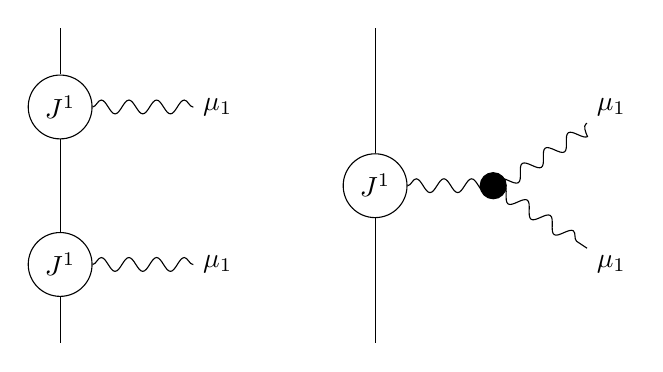
\begin{tikzpicture}
	\begin{scope}
		\node[circle, draw] (J1) at (0,1) {$\til{J}^1$};
		\node[circle, draw] (J2) at (0,-1) {$\til{J}^1$};
		\node (A1) at (2,1)  {$\mu_1$};
		\node (A2) at (2,-1)  {$\mu_1$};
		\draw[decorate, decoration={snake}] (J1) --(A1);
		\draw[decorate, decoration={snake}] (J2) --(A2);
		\draw (0,2) -- (J1) --(J2) -- (0,-2); 
	\end{scope}	
	\begin{scope}[shift={(4,0)}];
		\node[circle, draw] (J) at (0,0) {$\til{J}^1$};
		\node (A1) at (3,1)  {$\mu_1$};
		\node (A2) at (3,-1)  {$\mu_1$};
		\node[circle,draw,fill=black, minimum size = 0.2pt]  (V) at (1.5,0) {};  
		\draw[decorate, decoration={snake}] (J) -- (1.5,0) --  (A1);
		\draw[decorate, decoration={snake}] (1.5,0) --(A2);
		\draw (0,2) -- (J)-- (0,-2);
	\end{scope}
	\end{tikzpicture}
	\caption{Cancellation of the gauge anomaly of these two diagrams leads to the equation for the self OPE of the currents $\til{J}^1[k,l]$. \label{fig:JJcancel}}
\end{figure}

\subsubsection{}

Similar computations lead to the following tree-level OPEs.
We have the $\til{J}^2 \til{J}^2$ OPE:
\[ 
		\til{J}^2[r,s](0)  \til{J}^2[k,l](z)
	\simeq \frac{1}{z} (l-s)  \til{J}^2 [r+k,s+l-1] (0) . 
\]
The $\til{J}^1 \til{J}^2$ OPE:
\[ 
	\til{J}^1[r,s] (0) \til{J}^2[k,l](z) \simeq - \frac{1}{z} s  \til{J}^1[r+k, l+s - 1] (0) + \frac{1}{z} k \til{J}^2[k+r-1,l+s] (0).
\]
And finally, the $\til{J}^2 \til{J}^1$ OPE:
\[ 
	\til{J}^2[r,s] (0) \til{J}^1[k,l](z) \simeq - \frac{1}{z} r  \til{J}^2[r+k-1, l+s ] (0)    + \frac{1}{z} l \til{J}^1[k+r,l+s-1] (0).   
\]

\subsubsection{}

The calculations so far have involved the OPEs of the ``off-shell'' operators $\til{J}^i[r,s]$.
To obtain the on-shell OPEs we apply the constraints in \eqref{eqn:onshell}, which for the $J$-type operators takes the form
\beqn\label{eqn:Jonshell}
	 	J[r,s] = r \til{J}^2[r-1,s] - s \til{J}^1[r,s-1] .
\eeqn

We find
\begin{multline}
	J[r,s] (0) J[k,l](z) =   \frac{1}{z} (l-s) k r  \til{J}^2 [k+r-2,l+s-1]   \\
	+ \frac{1}{z} ls(k-r) \til{J}^1[k+r-1, l+s-2] \\
	+  \frac{1}{z} r (r-1) l  \til{J}^2[r+k-2, l+s -1 ]    - \frac{1}{z} l (l-1) r \til{J}^1[k+r-1,l+s-2]  \\
	+ \frac{1}{z} k s(s-1)  \til{J}^1[r+k-1, l+s - 2]    - \frac{1}{z}k s  (k-1) \til{J}^2[k+r-2,l+s-1] 
\end{multline}

Collecting the terms, we find the right hand side is
\begin{align*} 
	&\frac{1}{z} \left( (l-s)kr + r (r-1) l - ks (k-1)     \right)  \til{J}^2 [k+r - 2, l +s - 1]  \\
	&+ \frac{1}{z} \left( ls (k-r) - l (l-1) r + k s (s-1)  \right) \til{J}^1 [ k + r -1, l + s - 2]. 
\end{align*}
Finally, using \eqref{eqn:Jonshell}
we find that the OPE involving the on-shell operators $J[r,s]$ takes the form 
\[ 
	J[r,s](0)J[k,l](z) = \frac{1}{z} (rl-ks)  J[r+k-1,l+s-1](0).     
\]
As above, on the right hand side all operators are evaluated at $z = 0$ and with the fermionic variables $\what{\eta}+\what{\eta}'$. 
Note that the operators $J[r,s]$ with $r + s = 2$ which are independent of $\what{\eta}$ satisfy the OPE of the $\mf{su}(2)$ Kac-Moody algebra at level zero.
We will get a nontrivial level once we include the contribution from the back reaction, which we do in \S \ref{sec:br}. 

In the case that the hyper K\"ahler surface we compactify type IIB supergravity on is $T^4$ (instead of $K3$ which we have mostly considered in this paper), it is shown in \cite{CP} that the mode algebra corresponding to this full collection of OPE's of the $J$-operators can be expressed as the super loop space of the Lie algebra $\fw_{\infty}$ of Hamiltonoian vector fields on $\C^2$ \footnote{This is the quotient of the Lie algebra of functions on $\C^2$, which equipped with the standard Poisson bracket, by its center consisting of the constant functions.}
This is the Lie algebra $\cL^{1|4} \fw_\infty$ whose elements have the form
\beqn
z^{n} f(w_1,w_2; \eta_a) \in \cL^{1|4} \fw_\infty
\eeqn
for $n \in \Z$, where $f(w_1,w_2;\eta_a) \in \C[w_1,w_2] \slash \C \otimes \C[\eta_a]$. (Here, the $\eta_a, a=1,2,3,4$ variables generator the cohomology of $T^4$, so are fermionic.)
The super bracket is 
\beqn
[z^n f, z^m g] = z^{n+m} \eps^{ij} \del_{w_i} f \del_{w_j}g .
\eeqn

In the $K3$ case the mode algebra of the $J$-operators gives rise to a similar infinite-dimensional Lie algebra that we denote $L^{K3}\fw_\infty$.
Elements in this Lie algebra have the form
\beqn
z^{n} f(w_1,w_2; \eta) \in L^{K3}\fw_\infty 
\eeqn
where $n \in \Z$ and $f \in \C[w_1,w_2] \slash \C \otimes A$.
The super bracket is identical 
\beqn
[z^n f, z^m g] = z^{n+m} \eps^{ij} \del_{w_i} f \del_{w_j}g .
\eeqn

\subsection{$TJ$ OPE}

We turn to the tree-level OPE between the on-shell operators $T$ and $J$. 
First, we compute the tree-level OPE between the off-shell operators $\til{J}$ and $\til{T}$. 

The coefficient of $\til{J}^1$, for instance, in this OPE will be determined by the terms in the BRST variation of $\mu_1$ which involve $\fc_1$ and $\mu_z$ or $\fc_z$ and $\mu_1$. 
We collect such terms in the gauge variation of \eqref{eqn:j1vary} and 
\begin{equation}\label{eqn:Tvary}
\int_{(z,\eta_a) \in \C^{1|4}} \til{T} [m,n] (z,\eta_a) D_{m,n} \mu_z(z, w_i=0, \eta_a) .
\end{equation}
Recall that the gauge variation of $\mu_z$ is
\begin{align*}
Q \mu_z & = \dbar \fc_z + \mu_i \partial_{w_i} \fc_z + \mu_z \partial \fc_z - \fc_i \partial_{w_i} \mu_z - \fc_z \partial_z \mu_z \\
& -\epsilon_{ij} \partial_i \fc_\gamma \partial_j \alpha - \epsilon_{ij} \partial_i \fc_\alpha \partial_j \gamma .
\end{align*}
For now, we can disregard the terms involving $\alpha$ and $\fc_\gamma$ or $\fc_\alpha$ and $\gamma$.

The terms in the variations of \eqref{eqn:j1vary} and \eqref{eqn:Tvary} involving $\fc_1$ and $\mu_z$ or $\fc_z$ and $\mu_1$ is
\begin{align*}
& \int_{z, \eta} \til{J}^1[m,n](z,\eta_a) D_{m,n} (\mu_z \partial_{z} \fc_1 - \fc_z \partial_z \mu_1) (z, w_i=0,\eta_a) \\
+ & \int_{z,\eta} \til{T} [m,n](z,\eta_a) D_{m,n}(\mu_1 \partial_{w_1} \fc_z - \fc_1 \partial_{w_1} \mu_z) (z, w_i=0, \eta_a).
\end{align*}
The coefficient of $\fc_z$ can only be cancelled by a gauge variation of 
\[
\int_{z,z',\eta_a,\eta_a'} \til{J}^1 [r,s] (z,\eta_a) D_{r,s} \mu_1(z,w_i=0,\eta_a) \til{T} [k,l] (z',\eta_a') D_{k,l} \mu_z(z',w_i'=0,\eta_a') .
\]
By similar manipulation as above, we find that the gauge variation of this expression is 
\begin{align*}
& \int_{z,z',\eta_a,\eta_a'} \dbar_{z} \left(\til{J}^1 [r,s] (z,\eta_a) \til{T}[k,l](z',\eta_a')\right) D_{r,s} \fc_1 (z,w_i=0,\eta_a) D_{k,l} \mu_z (z',w'_i=0,\eta_a') \\
+ & \int_{z,z',\eta_a,\eta_a'} \dbar_{z'} \left(\til{J}^1 [r,s] (z,\eta_a) \til{T}[k,l](z',\eta_a')\right) D_{r,s} \mu_1 (z,w_i=0,\eta_a) D_{k,l} \fc_z (z',w'_i=0,\eta_a').
\end{align*}

To constrain the OPEs, we use the test functions $\mu_z = 0$, $\fc_1 = 0$, $\mu_1 = G(z,\zbar,\eta_a) \d \zbar w_1^k w_2^l$, 
$\fc_z = H(z,\zbar,\eta_a) w_1^r w_2^s$
for $G,H$ arbitrary smooth functions of the variables $z,\zbar,\eta_a$.
This yields the anomaly cancellation condition
\begin{multline}
\int_{z,z',\eta_a,\eta_a'} \dbar_{z'}\left(\til{J}^1 [r,s] (z,\eta_a) \til{T}[k,l](z',\eta_a')\right) G(z,\zbar,\eta_a) H(z',\zbar', \eta_a') = \\
- \int_{z'', \eta_a''} \til{J}^1[r+k, s+l] (z'', \eta_a'') H(z'', \zbar'', \eta_a'') \partial_{z''} G(z'', \zbar'', \eta_a'') \\ 
+ r \int_{z'',\eta_a''} \til{T}[r+k-1, s+l] (z'',\eta_a'') G(z'',\zbar'', \eta_a'') H(z'',\zbar'', \eta_a'') .
\end{multline}
Integrating the right hand side by parts gives us
\begin{multline}
\int_{z'', \eta_a''} \partial_{z''} \til{J}^1[r+k, s+l] (z'', \eta_a'') H(z'', \zbar'', \eta_a'') G(z'', \zbar'', \eta_a'') \\ +  \int_{z'', \eta_a''} \til{J}^1[r+k, s+l] (z'', \eta_a'') \partial_{z''} H(z'', \zbar'', \eta_a'')  G(z'', \zbar'', \eta_a'') \\
+ r \int_{z'',\eta_a''} \til{T}[r+k-1, s+l] (z'',\eta_a'') G(z'',\zbar'', \eta_a'') H(z'',\zbar'', \eta_a'') 
\end{multline}

Because $G,H$ are arbitrary functions, we arrive at the OPE
\begin{multline}
\til{T}[r,s](0,\eta_a) \til{J}^1[k,l] (z,\eta_a') \simeq \delta_{\eta_a=\eta_a'} \frac1z \partial_z \til{J}^1[r+k,s+l](0,\eta_a) + \delta_{\eta_a=\eta_a'} \frac{1}{z^2} \til{J}^1[r+k,s+l](0,\eta_a) \\ + r \delta_{\eta_a=\eta_a'} \til{T}[r+k-1,s+l] (0,\eta_a).
\end{multline}
Switching the $\eta_a$ variables to $\what{\eta}^a$ variables by applying the odd Fourier transform we can write this OPE as
\begin{multline}
\til{T}[r,s](0,\what{\eta}^a) \til{J}^1[k,l] (z,\what{\eta}'^a) \simeq \frac1z \partial_z \til{J}^1[r+k,s+l](0,\what{\eta}^a + \what{\eta}'^a) + \frac{1}{z^2} \til{J}^1[r+k,s+l](0,\what{\eta}^a + \what{\eta}'^a)  \\ + r \til{T}[r+k-1,s+l] (0,\what{\eta}^a + \what{\eta}'^a) .
\end{multline}

\subsubsection{}

In a completely similar way one can deduce the $\til{T} \til{J}^2$ OPE
\begin{multline}
\til{T}[r,s](0,\what{\eta}^a) \til{J}^2[k,l] (z,\what{\eta}'^a) \simeq \frac1z \partial_z \til{J}^2[r+k,s+l](0,\what{\eta}^a + \what{\eta}'^a) + \frac{1}{z^2} \til{J}^2[r+k,s+l](0,\what{\eta_a} + \what{\eta_a}')  \\ + s \til{T}[r+k,s+l-1] (0,\what{\eta}^a + \what{\eta}'^a) .
\end{multline}

\subsubsection{}

Using the $\til{T} \til{J}^i$ and $\til{J}^i \til{J}^2$ OPE's that we have computed, we deduce the OPE's between the on-shell operators $T$ and $J^i$ using \eqref{eqn:onshell}.
%\begin{equation} 
%	\begin{split}
%		T[r,s] &:=  \til{T}[r,s] - \frac{1}{2(r+1)} \partial_z \til{J}^1[r+1,s] - \frac{1}{2(s+1)} \partial_z \til{J}^2[r,s+1] \\
%		J[k,l] &:= k \til{J}^2[k-1,l] - l \til{J}^1[k,l-1] 
%	\end{split}
%\end{equation}
After some algebraic manipulation, we find
\begin{multline}
J[m, n](0)T[r, s](z) \simeq (nr-ms) { 1\over z}T[m + r -1, n + s -1](0) \\ + {1 \over z^2}\left({m \over 2(r + 1)} + {n \over 2(s + 1)}\right)J[m + r, n + s](0)
+{1 \over 2 z}\left({m \over m + r} + {n \over n + s} \right)\partial_z J[m + r, n + s](0)
\end{multline}
%\begin{multline}
%T[r,s](0, \eta_a) J[k,l](z,\what\eta'^a) \simeq \\ k \til{T}[r,s](0, \eta_a) \til{J}^2[k-1,l] - l \til{T}[k,l](0, \eta_a) \til{J}^1[k,l-1]  \\
%- \frac{k}{2(r+1)} \partial_z \til{J}^1[r+1,s] (0,\eta_a) \til{J}^2[k-1,l] + \frac{l}{2(r+1)} \partial_z \til{J}^1[r+1,s] \til{J}^1[k,l-1] \\
%- \frac{k}{2(s+1)} \partial_z \til{J}^2[r+1,s] (0,\eta_a) \til{J}^2[k-1,l] + \frac{l}{2(s+1)} \partial_z \til{J}^2[r+1,s] \til{J}^1[k,l-1] .
%\end{multline}
On the right hand side, all operators are evaluated at the variables $\what{\eta} +\what{\eta}'$.  We have dropped this dependence for clarity.

\subsection{$TT$ OPE}
\label{sec:TT1}

Following the same logic we constrain the $\til{T}\til{T}$ OPE. 
These OPE's are determined by terms in the BRST variation of $\mu_z$ which involve $c_z$ and $\mu_z$. 

Proceeding as above we set
\begin{align*}
\mu_z & = G(z,\zbar,\eta_a) \d \zbar w_1^k w_2^l \\
\mf{c}_1 & = H(z,\zbar,\eta_a) w_1^r w_2^s
\end{align*}
to arrive at the anomaly constraint
\begin{multline}
\int_{z,z',\eta_a,\eta_a'} \dbar_{z'} \left(\til{T}[r,s](z,\eta_a) \til{T}[k,l](z',\eta_a') \right) G(z,\zbar,\eta_a) H(z',\zbar',\eta_a') \\
= \int_{z'',\eta''_a} \til{T} [r+k, s+l]  (z'', \eta_a'') \left(G(z'',\zbar'', \eta_a'') \partial_{z''} H(z'', \zbar'', \eta_a'') - H(z'', \zbar'', \eta_a'') \partial_{z''} G(z'',\zbar'', \eta_a'') \right) 
\end{multline}

Integrating by parts and switching to the Fourier dual odd coordinates, we find the OPE 
\begin{equation}\label{ope:TT}
\til{T}[r,s] (0,\what\eta^a) \til{T}[k,l] (z, \what\eta'^a) \simeq \frac1z \partial_z \til{T}[r+k, s+l]  (0,\what\eta^a + \what\eta'^a) + 2 \frac{1}{z^2} \til{T}[r+k, s+l]  (0,\what\eta^a + \what\eta'^a) .
\end{equation}

\subsubsection{}

Using the $\til{T} \til{T}$ and $\til{J}^i \til{J}^j$ OPE's that we have computed, we deduce the OPE's between the on-shell operator $T$ and itself using \eqref{eqn:onshell}.
%\begin{equation} 
%	\begin{split}
%		T[r,s] &:=  \til{T}[r,s] - \frac{1}{2(r+1)} \partial_z \til{J}^1[r+1,s] - \frac{1}{2(s+1)} \partial_z \til{J}^2[r,s+1] \\
%		J[k,l] &:= k \til{J}^2[k-1,l] - l \til{J}^1[k,l-1] 
%	\end{split}
%\end{equation}
After some algebraic manipulation, we find
\beqn
\begin{aligned}[]
T[m, n](0)T[r, s](z) &\sim {1 \over z}\left(1 + {r \over 2(m+1)} + {s \over 2(n+1)}\partial_z \right) T[m + r, n +s](0) \\ \nonumber &+ {1 \over z^2}\left(2 + {r \over 2(m+1)} + {s \over 2(n+1)} + {m \over 2(r+1)} + {n \over 2(s+1)} \right)T[m + r, n + s](0)\\
&+{1 \over 4 z}\left({1 \over (m + 1)(n + s + 1)}- {1 \over (n +1)(m + r + 1)} \right) \partial^2_z J[m + r  +1, n + s +1](0) \\ 
&+{1 \over 4 z^2}\left({1 \over (m + 1)(s + 1)}- {1 \over (n+1)(r + s)}\right)\partial_z J[m + r + 1, n + s + 1](0) \\  
&+ {1 \over 4 z^2}\left({1 \over n + s + 1}({2 + m + r \over (1 + m)(1 + r)}) - {1 \over m + r + 1}({2 + n + s \over (1 + n)(1 + s)}) \right) \\  & \ \ \ \ \ \ \ \ \ \ \ \ \ \ \ \ \ \partial_z J[m + r + 1, n + s + 1](0) \\ 
&+{1 \over 2 z^3}\left( {1 \over (m + 1)(s + 1)}- {1 \over (n+1)(r + s)}\right) J[m + r + 1, n + s + 1](0) \\ 
\end{aligned}
\eeqn
On the right hand side, all operators are evaluated at the variables $\what{\eta} +\what{\eta}'$.  We have dropped this dependence for clarity.

\subsection{$GG$ OPE}
To constrain the $G_\alpha$, $G_\gamma$ OPE we consider terms in the gauge variations of the classical couplings involving $\alpha$ and $\fc_\gamma$ or $\gamma$ and $\fc_\alpha$ (we have disregarded those terms in the analysis above as they played no role in the previous OPE calculations).

The term in the gauge variation of $\mu_i$ involving the fields $\alpha$ and $\fc_\gamma$ is $\epsilon_{ij} \partial_j \fc_\gamma \partial_z \alpha - \epsilon_{ij} \partial_z \fc_\gamma \partial_j \alpha.$
Therefore, the gauge variation of $\int \til{J}^i [m,n] D_{m,n} \mu_i$ involving such terms is
\[
\int \til{J}^i [m,n] D_{m,n} \left( \epsilon_{ij} \partial_{w_j} \fc_\gamma \partial_z \alpha - \epsilon_{ij} \partial_z \fc_\gamma \partial_{w_j} \alpha \right) .
\]
%It will be useful to integrate by parts to write this expression as
%\begin{align*}
%& \int \til{J}^i [m,n] D_{m,n} \left(-\epsilon_{ij} (\partial_{w_j} \partial_z \fc_\gamma) \alpha - \epsilon_{ij} \partial_z \fc_\gamma \partial_{w_j} \alpha \right) \\
%& + \int \epsilon_{ij} \partial_{z} \til{J}^i [m,n] D_{m,n} \partial_{w_j} \fc_\gamma \alpha 
%\end{align*}
%so that all $z$-derivatives act on $\fc_\gamma$ or $\til{J}[m,n]$. 

The term in the gauge variation of $\mu_z$ involving $\alpha$ and $\fc_\gamma$ is $-\epsilon_{ij} \partial_{w_i} \fc_\gamma \partial_{w_j} \alpha.$
Therefore, the gauge variation of $\int \til{T}[m,n] D_{m,n} \mu_z$ involving such terms is
\[
\int \til{T}[m,n] D_{m,n} (- \epsilon_{ij} \partial_{w_i} \fc_\gamma \partial_{w_j} \alpha) .
\]

The sum of these anomalies can only be cancelled by a gauge variation of a term of the form
\[
\int_{z,z',\eta_a,\eta_a'} G_\alpha[r,s] (z,\eta_a) D_{r,s} \alpha(z,w_i=0,\eta_a) G_\gamma[k,l] (z',\eta_a') D_{k,l} \gamma (z',w_i'=0,\eta_a') .
\]
The gauge variation of this expression involving the terms $\fc_\gamma$ and $\alpha$ is
\[
\int_{z,z',\eta_a,\eta_a'} \dbar_{z'} \left(G_\alpha[r,s] (z,\eta_a) G_\gamma[k,l] (z',\eta_a')\right) D_{r,s} \alpha(z,w_i=0,\eta_a) D_{k,l} \fc_\gamma (z',w_i'=0,\eta_a) .
\]

Let us plug in test fields $\alpha = \d \zbar w_1^r w_2^s G(z,\zbar,\eta_a)$ and $\fc_\gamma = w_1^k w_2^l H(z,\zbar, \eta_a)$ where $G,H$ are arbitrary functions.  
Cancellation of these gauge anomalies requires
\begin{multline}
\int_{z,z',\eta_a,\eta_a'} \dbar_{z'} \left(G_\alpha[r,s] (z,\eta_a) G_\gamma[k,l] (z',\eta_a')\right) G(z,\zbar, \eta_a) H(z',\zbar',\eta_a') = \\ l \int_{z'',\eta_a''} \til{J}^1[r+k,s+l-1] (z'',\eta_a'') H(z'',\zbar'', \eta_a'') \partial_{z''} G(z'', \zbar'', \eta_a'') \\
- k \int_{z'',\eta_a''} \til{J}^2[r+k-1,s+l] (z'',\eta_a'') H(z'',\zbar'', \eta_a'') \partial_{z''} G(z'', \zbar'', \eta_a'') \\
-s \int_{z'',\eta_a''} \til{J}^1[r+k,s+l-1] (z'',\eta_a'') \partial_{z''} H(z'',\zbar'', \eta_a'')  G(z'', \zbar'', \eta_a'') \\
+ r \int_{z'',\eta_a''} \til{J}^2[r+k-1,s+l] (z'',\eta_a'') \partial_{z''} H(z'',\zbar'', \eta_a'') G(z'', \zbar'', \eta_a'') \\
- \int_{z'',\eta_a''} \til{T}[r+k-1,s+l-1] (z'',\eta_a'') H(z'',\zbar'',\eta_a'') G(z'',\zbar'', \eta_a'') .
\end{multline}
We integrate by parts to rewrite the right hand side as
%\begin{multline}
%-l \int_{z'',\eta_a''} \partial_{z''} \til{J}^1[r+k,s+l-1] (z'',\eta_a'') H(z'',\zbar'', \eta_a'') G(z'', \zbar'', \eta_a'') \\ - l \int_{z'',\eta_a''} \til{J}^1[r+k,s+l-1] (z'',\eta_a'') \partial_{z''} H(z'',\zbar'', \eta_a'') G(z'', \zbar'', \eta_a'') \\
%+ k \int_{z'',\eta_a''} \partial_{z''}\til{J}^2[r+k-1,s+l] (z'',\eta_a'') H(z'',\zbar'', \eta_a'') G(z'', \zbar'', \eta_a'') 
%\\
%+ k \int_{z'',\eta_a''} \til{J}^2[r+k-1,s+l] (z'',\eta_a'') \partial_{z''} H(z'',\zbar'', \eta_a'') G(z'', \zbar'', \eta_a'') 
%\\
%-s \int_{z'',\eta_a''} \til{J}^1[r+k,s+l-1] (z'',\eta_a'') \partial_{z''} H(z'',\zbar'', \eta_a'')  G(z'', \zbar'', \eta_a'') \\
%+ r \int_{z'',\eta_a''} \til{J}^2[r+k-1,s+l] (z'',\eta_a'') \partial_{z''} H(z'',\zbar'', \eta_a'') G(z'', \zbar'', \eta_a'') \\
%- \int_{z'',\eta_a''} \til{T}[r+k-1,s+l-1] (z'',\eta_a'') H(z'',\zbar'',\eta_a'') G(z'',\zbar'', \eta_a'') .
%\end{multline}
\begin{multline}
\int_{z'',\eta_a''} \bigg( -l \partial_{z''} \til{J}^1[r+k,s+l-1] + k \partial_{z''} J[r+k-1,s+l] \\  - \til{T}[r+k-1, s+l-1]\bigg) (z'',\eta_a'') H(z'',\zbar'', \eta_a'') G(z'', \zbar'', \eta_a'') \\ - (s+l) \int_{z'',\eta_a''} \til{J}^1[r+k,s+l-1] (z'',\eta_a'') \partial_{z''} H(z'',\zbar'', \eta_a'') G(z'', \zbar'', \eta_a'')
\\
+ (r+k) \int_{z'',\eta_a''} \til{J}^2[r+k-1,s+l] (z'',\eta_a'') \partial_{z''} H(z'',\zbar'', \eta_a'') G(z'', \zbar'', \eta_a'') .
\end{multline}

From these expressions we can read off the OPE's just as above. 
We obtain
\begin{multline}
G_{\alpha} [r,s] (0,\what\eta_a) G_{\gamma}[k,l](z,\what\eta_a') \simeq  - (s+l) \frac{1}{z^2} \til{J}^1[r+k, s+k-1] + (r + k) \frac1{z^2} \til{J}^2 [r+k-1, s+l] \\
- l \frac1z \partial_z \til{J}^1[r+k, s+l-1] + k \frac1z\partial_z \til{J}^2 [r+k-1, s+l]
+(rl-sk) \frac1z \til{T}[r+k-1, s+l-1] .
\end{multline}

\subsubsection{}

Using \eqref{eqn:onshell} we obtain the on-shell $G^\alpha-G^\gamma$ OPE's
\beqn
\begin{aligned}[]
G^{\alpha}[m, n](0)G^{\gamma}[r, s](z) &\sim {(nr-ms) \over z}T[m + r -1, n + s -1](0) + {1 \over z^2}J[m + r, n + s](0) \\ \nonumber
&+{1 \over z}\left(({m \over 2 (m + r)} + {n \over 2 (n + s)})\right)\partial_z J[m + r, n+s](0)
\end{aligned}
\eeqn
On the right hand side, all operators are evaluated at the variables $\what{\eta} +\what{\eta}'$.



\subsection{$TG$ OPE}

The $TG$ OPE can be computed similarly. We record the result in the next section.

\subsection{Tree-level on-shell OPEs}

The OPE's we have just computed completely characterize the tree-level defect chiral algebra.
In the final part of this section we summarize all tree-level OPE's that we have deduced above.
In the next section we will characterize loop effects which modify this tree-level chiral algebra.

\textcolor{red}{NP: note, we should carefully check signs and normalizations against the N=4 superconformal algebra, etc.}
\textcolor{red}{NP: it may be prettier to separate the $J[m,n]$ OPEs when one or both arguments are zero from the rest, to avoid using the clunky theta function notation.}

If $nr-ms > 0$ the OPEs are
\begin{align}
J[m,n](0)J[r, s](z) &\sim {(nr-ms) \over z}J[m + r -1, n + s -1](0) \\
J[m, n](0)T[r, s](z) &\sim {(nr-ms) \over z}T[m + r -1, n + s -1](0) + {1 \over z^2}\left({m \over 2(r + 1)} + {n \over 2(s + 1)}\right)J[m + r, n + s](0) \\ \nonumber
&+{1 \over 2 z}\left({m \over m + r} + {n \over n + s} \right)\partial_z J[m + r, n + s](0)\\
G[m, n](0)J[r, s](z) &\sim {(ms - rn) \over z}G[m + r -1, n + s - 1](z) \\
G[m, n](0)T[r, s](z) &\sim ({1 \over z} \partial_z + {1 \over z^2})G[m + r, n+s](0) + \left({m \over 2(r+1)} + {n \over 2 (s + 1)}\right){1 \over z^2}G[m + r, n+s](0) \\
T[m, n](0)T[r, s](z) &\sim {1 \over z}\left(1 + {r \over 2(m+1)} + {s \over 2(n+1)}\partial_z \right) T[m + r, n +s](0) \\ \nonumber &+ {1 \over z^2}\left(2 + {r \over 2(m+1)} + {s \over 2(n+1)} + {m \over 2(r+1)} + {n \over 2(s+1)} \right)T[m + r, n + s](0)\\ \nonumber
&+{1 \over 4 z}\left({1 \over (m + 1)(n + s + 1)}- {1 \over (n +1)(m + r + 1)} \right) \partial^2_z J[m + r  +1, n + s +1](0) \\ \nonumber
&+{1 \over 4 z^2}\left({1 \over (m + 1)(s + 1)}- {1 \over (n+1)(r + s)}\right)\partial_z J[m + r + 1, n + s + 1](0) \\ \nonumber 
&+ {1 \over 4 z^2}\left({1 \over n + s + 1}({2 + m + r \over (1 + m)(1 + r)}) - {1 \over m + r + 1}({2 + n + s \over (1 + n)(1 + s)}) \right) \\ \nonumber & \ \ \ \ \ \ \ \ \ \ \ \ \ \ \ \ \ \partial_z J[m + r + 1, n + s + 1](0) \\ \nonumber
&+{1 \over 2 z^3}\left( {1 \over (m + 1)(s + 1)}- {1 \over (n+1)(r + s)}\right) J[m + r + 1, n + s + 1](0) \\ \nonumber
G^{\alpha}[m, n](0)G^{\gamma}[r, s](z) &\sim {(nr-ms) \over z}T[m + r -1, n + s -1](0) + {1 \over z^2}J[m + r, n + s](0) \\ \nonumber
&+{1 \over z}\left(({m \over 2 (m + r)} + {n \over 2 (n + s)})\right)\partial_z J[m + r, n+s](0)
\end{align}. 

The coefficients in the OPEs between $J-T$ and $G-G$ have to be treated with slightly more care for special choices of $n, r, m, s$, though the basic structure of the OPEs is the same.
For the $J-T$ OPE, the above expression also holds when $nr - ms = 0$ and $nr = m s >0$. 
For the $G-G$ OPE, if $n r - ms = 0$ and $nr = ms > 0$ we have
\begin{align}
G^{\alpha}[m, n](0)G^{\gamma}[r, s](z) &\sim {(nr-ms) \over z}T[m + r -1, n + s -1](0) + {1 \over z^2}J[m + r, n + s](0) \\ \nonumber
&+{1 \over z}\partial_z J[m + r, n+s](0).
\end{align}
The remaining cases are as follows. If $nr-ms = 0$ and $n r = ms = 0$ the TJ and GG OPE coefficients are instead as follows. \newline
If $r = m = 0, s \neq 0$:
\begin{align}
J[m, n](0)T[r, s](z) &\sim {1 \over z^2}\left({n \over 2(s + 1)}\right)J[m + r, n + s](0) +{1 \over 2 z}\left({n \over n + s} \right)\partial_z J[m + r, n + s](0) \\ \nonumber
G^{\alpha}[m, n](0)G^{\gamma}[r, s](z) &\sim {1 \over z^2}J[m + r, n + s](0) +{1 \over z}\left({n \over  (n + s)}\right)\partial_z J[m + r, n+s](0)
\end{align}
If $n = s = 0, r \neq 0$:
\begin{align}
J[m, n](0)T[r, s](z) &\sim {1 \over z^2}\left({m \over 2(r + 1)}\right)J[m + r, n + s](0) +{1 \over 2 z}\left({m \over m + r} \right)\partial_z J[m + r, n + s](0)\\
G^{\alpha}[m, n](0)G^{\gamma}[r, s](z) &\sim {1 \over z^2}J[m + r, n + s](0) +{1 \over z}\left({m \over m + r}\right)\partial_z J[m + r, n+s](0)
\end{align}
If $r = s= 0$ (note that there are no G operators for these values):
\begin{align}
J[m, n](0)T[r, s](z) &\sim {1 \over 2 z^2}\left(m + n\right)J[m + r, n + s](0) +{1 \over  z}\partial_z J[m + r, n + s](0)
\end{align}
\textcolor{red}{NP: Probably some of these can be written better with epsilon symbols and Pauli matrices to account for their $SU(2)$ reps, as in the N=4 SCA?}

We have so far discussed OPEs that come from cancelling the BRST variation of bulk/defect Feynman diagrams that have the topology of tree diagrams. However, they do not yet constitute the complete planar, i.e. $N \rightarrow \infty$, chiral algebra. In particular, we have not accounted for the effects of backreaction, which will serve to deform and centrally extend the planar algebra. If we perform the rescaling of the Kodaira-Spencer Lagrangian in the backreacted geometry, as discussed in section \ref{}, then the diagrammatics have the following dependence on $N$: 
\begin{enumerate}
\item The Kodaira--Spencer Lagrangian scales like $\sim N$. \\
\item The term in the Lagrangian implementing the backreaction, i.e. the cubic vertex coupling Kodaira--Spencer theory to the defect, scales like $\sim N$. \\
\item The propagator (either in the form of bulk-bulk or bulk-defect propagators) scales like $N^{-1}$.
\end{enumerate}

Putting this together, we find that the same class of diagrams as in \cite{CP} survive in the planar limit. We reproduce these below in Figure \ref{fig:alldiagramsplanar}. As expected, this leads to central terms scaling like the CFT central charge $c \sim N$, as well as a new class of diagrams arising from the backreaction that do not scale with $N$ and deform the algebra. 
In the next section, we turn now to computing these diagrams and completing our characterization of the planar chiral algebra from Koszul duality. 

To compute non-planar corrections, one would need to repeat this procedure for a larger class of bulk diagrams including: 1) diagrams with loops in the bulk, and 2) diagrams with $\leq 2$ backreaction legs attached to the defect plus an arbitrary number of bulk-defect propagators. The integrals quickly get difficult when working beyond the box topology, but we remark that an impressive class of non-planar contributions to the OPE of two open-string bulk operators (that is, considering additional space-filling D-branes coupled to Kodaira--Spencer theory), has been computed in \cite{Keyou} by incorporating a refined model for Kaluza--Klein reduction via homotopy transfer.
These corrections, valid for a chiral algebra dual to Kodaira-Spencer type theories plus space-fillng D-branes, can be appended immediately to our chiral algebra, but does not yet include any dependence on the fermionic variables of the internal compactification manifold. 
One can view the non-planar contributions of \cite{Keyou} as incorporating diagrams of the second type (i.e. those without bulk loops). 
It would be very interesting to understand if other techniques from homological algebra can be leveraged to more directly obtain other non-planar contributions. 

\begin{figure}



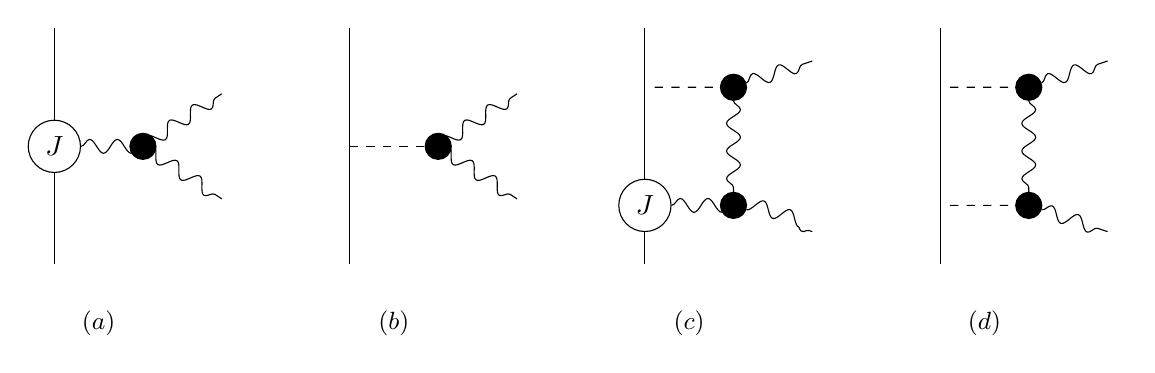
\begin{tikzpicture}[scale={0.75}]
		


	\begin{scope}[shift={(-5,0)}]
		\node[circle, draw] (J) at (0,0) {$J$};
		\node (A1) at (3,1)  {};
		\node (A2) at (3,-1)  {};
		\node[circle,draw,fill=black, minimum size = 0.2pt]  (V) at (1.5,0) {};  
		\draw[decorate, decoration={snake}] (J) -- (1.5,0);
		\draw[decorate, decoration={snake}] (1.5,0) --(A1);
		\draw[decorate, decoration={snake}] (1.5,0) --(A2);
		\draw (0,2)-- (J) -- (0,-2);
		\node at (0.75,-3) {\small $(a)$};
	\end{scope}


	\begin{scope}[shift={(0,0)}];
	%	\node[circle, draw] (J) at (0,0) {$J$};
		\node (A1) at (3,1)  {};
		\node (A2) at (3,-1)  {};
		\node[circle,draw,fill=black, minimum size = 0.2pt]  (V) at (1.5,0) {};  
		\draw[dashed] (0,0) -- (1.5,0);
		\draw[decorate, decoration={snake}] (1.5,0) --(A1);
		\draw[decorate, decoration={snake}] (1.5,0) --(A2);
		\draw (0,2)-- (0,-2);
		\node at (0.75,-3) {\small $(b)$};
	\end{scope}



	\begin{scope}[shift={(5,0)}]
		\node (J1) at (0,1) {};
		\node[circle, draw] (J2) at (0,-1) {$J$};
		\node (A1) at (3,1.5)  {};
		\node (A2) at (3,-1.5)  {};

		\node[circle,draw,fill=black ]  (V1) at (1.5,1) {}; 
		\node[circle,draw,fill=black]  (V2) at (1.5,-1) {};  
		\draw[decorate, decoration={snake}]  (V1) --  (A1);
		\draw[decorate, decoration={snake}] (J2) -- (V2) -- (A2);
		\draw[decorate, decoration={snake}] (V1) -- (V2);
		\draw[dashed] (J1) to (V1);
		\draw (0,2) --  (J2) -- (0,-2);
		\node at (0.75,-3) {\small $(c)$};
	\end{scope}


	\begin{scope}[shift={(10,0)}]
		\node (J1) at (0,1) {};
		\node (J2) at (0,-1) {};
		\node (A1) at (3,1.5)  {};
		\node (A2) at (3,-1.5)  {};

		\node[circle,draw,fill=black ]  (V1) at (1.5,1) {}; 
		\node[circle,draw,fill=black]  (V2) at (1.5,-1) {};  
		\draw[decorate, decoration={snake}]  (V1) --  (A1);
		\draw[decorate, decoration={snake}] (V2) -- (A2);
		\draw[dashed] (J1)--(V1);
		\draw[dashed] (J2)--(V2);
		\draw[decorate, decoration={snake}] (V1) -- (V2); 
		\draw (0,2)  -- (0,-2);
		\node at (0.75,-3) {\small $(d)$};
	\end{scope}


	\end{tikzpicture}
	\caption{All diagrams that contribute in the planar limit.  Diagrams $(a)$ and $(c)$ scale like $\sim \mathcal{O}(1)$ in the large-$N$ limit, and comprise 3-pt functions. We have computed the chiral algebra OPEs arising from Diagrams $(a)$ in this section. Diagrams $(b)$ and $(d)$ scale like $\sim \mathcal{O}(N)$ in the  large-$N$ limit and contribute to the 2-pt function or central extension of the algebra (terms in the OPE proportional to the identity operator). \label{fig:alldiagramsplanar}}
\end{figure}



\end{document}
